\section{YouCook: modello del dominio}
\begin{figure}[H]
    \centering
 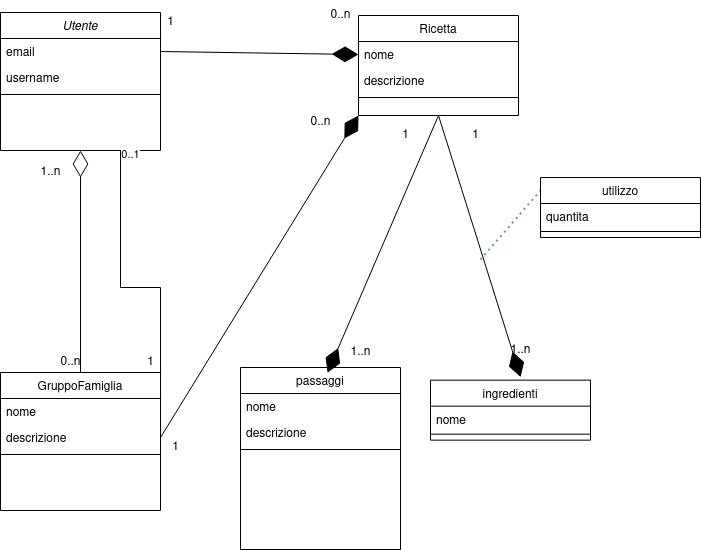
\includegraphics[scale=0.7]{resources/modello_del_dominio.drawio.png}
   \caption{Modello del dominio dell'applicazione}
\end{figure}
Il modello del dominio sopra rappresentato definisce le entità in gioco nell'applicazione. In particolare, vengono sfruttate due realazioni tra le classi utenti e gruppo famiglia per rappresentare i membri e il proprietario del gruppo. Viene inoltre utilizzata una classe d'associazione per rappresentare l'utilizzo del dato ingrediente in quella ricetta.